\documentclass[jou,apacite]{apa6}
%\usepackage[style=apa,backend=biber]{biblatex}

\title{Analysis of Speed Reading in Contemporary Literature}
\shorttitle{Does Rapid Serial Visual Presentation (RSVP) make us faster readers?}

\fourauthors{Mathias K. Berthelsen}{Gustav Dahl}{Benjamin N. Overgaard}{Andreas M. Thomsen}
\fouraffiliations{Aalborg University}{Aalborg University}{Aalborg University}{Aalborg University}


\abstract{This paper will investigate the speed reading technique known as Rapid Serial Visual Presentation (RSVP) as well as how it relates to other topics, e.g. eye movement and modes for reading. The goal of this paper is to analyze contemporary theory and literature and discuss the different points of view in regards to speed reading.}

\rightheader{APA style}
\leftheader{MTA 14737}

\begin{document}
\maketitle

% A category with the (minimum) three required fields
%\category{H.4}{Information Systems Applications}{Miscellaneous}
%A category including the fourth, optional field follows...
%\category{D.2.8}{Software Engineering}{Metrics}[complexity measures, performance measures]

%\terms{Perception, reading}

%\keywords{Speed reading, reading, RSVP, comprehension, eye saccades} % NOT required for Proceedings

\section{Introduction}
%BASED ON PRELIMIANARY RESEARCH, TOOLS SHOULD BE DEVELOPED WITH A MODULAR MINDSET AND ALLOW FOR TWEAKABLE PARAMTERS and stuff

%Describe basic concept of the product (context)
%We have a collaboration with TAW
%They make 3D point n click game
%Framing system
%Path system
\textbf{real world problem}
\textbf{Time based > interactive}
\textbf{Gap of knowledge}
\textbf{Opgaver / features er unclear, derfor bruger vi PD}

ANDREAS

This project is based on a collaboration between Medialogy and a group of artists from The Animation Workshop (TAW) in Viborg. As their bachelor project, the students at TAW developed a 3D point 'n click game, \textit{FEELS}, for the iPad using the Unity game engine. The TAW project spanned two semesters (pre-production and production), whereas this Medialogy project lasted only the first semester. Two additional programmers have also been working full-time on the project.

During the collaboration, it was decided that we should focus on developing a camera system for the game. This tool should empower the artists, so that the artists didn't have to worry about technical details. It should be simple to set up and function in a similar fashion as other 3D applications that the TAW students have been trained in during their three-year education. The camera tool was chosen, since it does not directly influence and interfere with the gameplay, making it easier for the other programmers to work directly on the game.

Before we began designing and implementing the tool, we conducted several preliminary studies to get an understanding of how game development tools should be made. We visited two game companies (KnapNok Games and Unity Studios), as well as conducting an online survey to gather, information about game development tools. The key findings were that the tool should be developed in a modular fashion and allow the user to tweak as many parameters as deemed necessary. Additional notes from the studies can be found in \textbf{APPENDIX X}.


There are many ways to design camera motions in games. Fundamentally, one can distinguish between \textit{cinematic sequences} and \textit{interactive gameplay}. These two are typically considered mutually exclusive, because cinematic sequences per definition is non-interactive \cite{haigh-hutchinson_real-time_2009}. However, it is also possible to mix those two, so the camera can dynamically adapt to certain things happening in the game, e.g., game events and player input. This means that a sequence does not have to be viewed in exactly the same way every time. For example, depending on the player's movement, the camera can change accordingly.

%Sometimes it might be necessary to put certain restrictions on where the player can move. An example of this could be a special "boss battle" where the player is confined in a restricted area. Typically, the camera would zoom out and focus on specific parts of this boss enemy (e.g. a weak point). The camera dynamically frames the scene in such a way so that the player and the enemy are visible at all times \cite{haigh-hutchinson_real-time_2009}.

Games often require the ability to replay previous sequences of the gameplay. This can be used to replicate certain events to re-create the motion and visual state of objects in a scene \cite{haigh-hutchinson_real-time_2009}. It can be achieved by recording the rendering state of objects on a set amount of frames, and then use \textit{interpolation} to calculate the state of said objects. Interpolation is a method of inserting intermediate values into a set of data and makes it possible to take sampled data and generate new points in between \cite{haigh-hutchinson_real-time_2009}. Replaying of this data can be referred to as \textit{keyframing}. Keyframing of camera data requires position and orientation of the camera, together with a time interval between the samples \cite{haigh-hutchinson_real-time_2009}.
\section{Background Knowledge}

\subsection{Eye movements}
To understand how speed reading is possible, it's important to understand some basics on how the eye moves.

When you read, visually analyse or look for something, your eyes are doing a series of movements called \textit{saccades}. In between these movements your eyes shortly fixate on elements, these stops called \textit{fixations}. Each fixations lasts only around 200-300 ms, so our eyes are quickly looking around a scene to find new details to fixate on. Luckily the movements of the eyes themselves are incredibly fast, reaching speeds of 500 degrees a second \cite{MATHIAS KILDE}.


But this all depends on what you're using your eyes for. There is generally three types of saccades: pursuit, vergence and vestibular. \textit{Pursuit} is when your eyes are trying to fixate on something moving. Generally, in these cases, the saccades are slower, as your eyes are following the target and not going back and forth between different targets \cite{KILDE MATHIAS}.
\textit{Vergence} is the inwards movement of your eyes to focus on something getting closer to you \cite{KILDE MATHIAS}.

\textit{Vestibular} movement is the eyes rotating to compensate for body and/or head movement. This is both caused by visual stimulation, but mostly by the vestibular organ in your ears. This is also also why your sight gets blurry when you're dizzy.

In the case of reading, it's also important to talk about the different kinds of small saccades the eyes are capable of. \textit{Nystagmus} is very tiny and quick movements in the eyes, which causes a kind of tremor in your vision \cite{KILDE MATHIAS}. You will notice it when staring intently at a fixed point. It's believed that this is a precaution in the eyes to make the nerve cells keep firing by continuously stimulating them. Furthermore, the eyes also experience small \textit{drifts}. These are believed to be the results of a less-than-perfect control of the oculomotor resulting in your eyes slowly drifting to one side. To accommodate this the eyes make tiny saccades, called \textit{microsaccades}, to realign themselves \cite{KILDE MATHIAS}.

Further, it's important to the understanding of reading is \textit{saccade latency}. Every time a saccade is made, some calculations are needed to approximate where to move the eyes to fixate on a desired target. Even if excluding the uncertainty of where to move the eyes, it would still take 150-175 ms for the initial "request" of moving the eyes to the actual start of the movement. Cognitive processes further increases this latency, but also increases accuracy, meaning your fixation falls closer to the point of interest.
\textbf{
(Gustav: maybe write something about cognitive processes from Perception book here)}

During the saccade, though, everything is a blur. Or it should be anyway. It seems certain parts associated with processing visual inputs are halted during saccades. This process is called \textit{saccadic suppression}. But this is independent of the lexical processing, which means a reader is able to process read text in parallel with saccades \cite{KILDE MATHIAS}.

A fixation is not needed to read a word though. Your attention can be shifted to objects or words in your peripheral vision. But it is not possible to make a saccade without shifting attention to the fixation.

\subsection{Optimal Recognition Position} \label{ORP}
The destination of each saccade when reading, or the fixation point, depends on the content of the sentence; sometimes, the eye also skip words by saccading past them. 80\% of the fixation points are on content words (nouns, verbs and adjectives) and the remaining 20\% are on articles, pronouns, and conjunctions \cite{eysenck_cognitive_2010}. The fixation point inside the words themselves, the \textit{optimal recognition position} (ORP), has an impact on how fast a reader can name the word they are looking at. Research has shown that the ORP is near the middle or slightly left of the middle \cite{oregan_optimal_1992, nazir_letter_1998, oregan_convenient_1984}. The added recognition time as the fixation point deviates from the ORP is a U-shaped curve, see Figure \ref{fig:ucurve}, with around 20 ms added for each letter of deviation.

\begin{figure}[htbp]
\centering
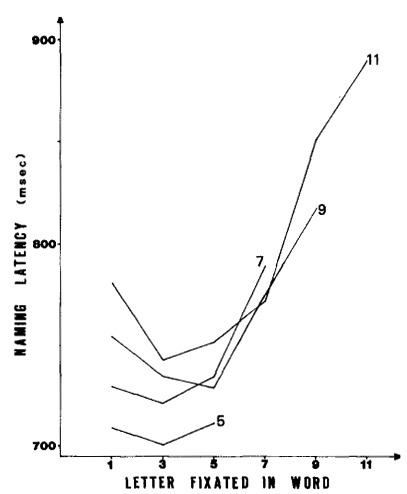
\includegraphics[width=0.4\textwidth]{Pics/ucurve}
\caption{The time it took participants to name the word they saw depending on their fixation point in the word. This graph shows results for words of length 5, 7, 9 and 11. \protect\cite{oregan_convenient_1984}}
\label{fig:ucurve}
\end{figure}

Removing the spacing between words decreases the reading speed with around 30\%. Fixation does not fall on the ORP but tends to the beginning of words. Splitting long words, like long Danish or German compound words, into their individual words, increases reading speed, even though it was grammatically incorrect. Likewise with putting in spaces in Thai, where there are no spaces.

\subsection{Meta-guiding reading (using a pen to keep focus)}
GUSTAV

\subsection{Modes for reading}
BENJAMIN

("gears" - depending on context, you switch "gear"):
Read for memorize
Read for learning
Rauding (sentential integration, lexical + semantic) - most optimal
Skimming (semantic encoding)
Scanning (lexical access? using memory)
Reading rate (WPM) - rauding is the best?
Cognitive speed vs. reading speed
E = AR (E: Efficiency, A: Accuracy, R: Rate)
=======
\subsection{Attention}
MATHIAS

\subsection{Reading Processes}
\citeA{carver_reading_1992} presents five reading processes, also referred to as \textit{gears} (see Figure \ref{fig:trace_cross}). Each gear is defined by its \textit{goal}, \textit{culminating component}, and its \textit{speed}, measured by \textit{WPM} (words per minute). WPM also varies based on reading level, so to block out this bias, \citeauthor{carver_reading_1992} bases his experiments exclusively on college students. The following section is based on his study.

\begin{figure*}[htbp]
\centering
\captionsetup{justification=centering}
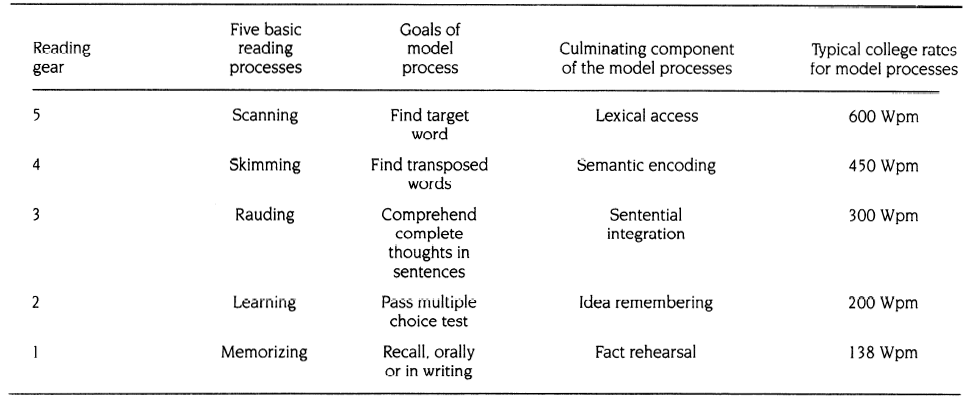
\includegraphics[width=1\textwidth]{Pics/gears_list}
\caption{Each gear has its own goal, culminating component, and WPM. \protect\cite{carver_reading_1992}}
\label{fig:gears_list}
\end{figure*}

The goal relies on the reader's intent when reading the text. For instance, the reader could read the text just to find a single word (scanning). The culminating component of a gear, is then the cognitive process that it requires. \textit{Lexical access} is the component used for finding a single word in memory. If the reader's goal changed to finding a certain sentence in the text, such as in skimming, transposed words must be found and the activity would require an additional component; \textit{semantic encoding}. Other than just finding the words, the reader must now determine the meaning of the sentence. In order for the reader to understand the complete thought of a sentence, the \textit{sentential integration} component must be added. These three components together are the requirement for the most basic and most used reading process - \textit{rauding}, also known as \textit{typical reading}. The word comes from a combination of 'auding' and 'reading', as they both share the same underlying comprehension processes. If the goal of reading the text is to learn, e.g., in order to answer a test, the \textit{idea remembering} component is added. In this gear, some words require re-reading and longer time to process. The final gear is focused around remembering the text and uses the \textit{fact rehearsal} component. This gear requires rehearsing the material and memorizing it. 
\citeA{carver_reading_1992} goes on to mention that the best readers shift up and down in gear while reading, based on the difficulty of the material - a term called \textit{process flexibility}. 

By having college students read a text followed by answering two multiple choice tests, as well as judging their own performance, \citeauthor{carver_reading_1992} tested efficiency at different reading rates. It was found that the students were most efficient at rates around 300 WPM - the rauding reading rate. This rate has therefore been referred to as the most optimal reading rate.
%Efficiency was calculated from the product of accuracy and reading rate, and the accuracy was determined through multiple-choice tests as well as self-judgement.

\citeauthor{carver_reading_1992} also mentions the term \textit{cognitive speed}, which acts as a limit of the reading speed. If the reader passes this limit, he will not be able to operate the culminating components successfully, resulting in a poor comprehension. The main concern however for most students is to make the reading speed reach the limit of the cognitive speed.

\textbf{(Gustav: maybe remove this quote?)}

\citeauthor{carver_reading_1992} describes how the \textit{rauding theory} relates to the \textit{schema theory}. The schema theory uses gears 1 and 2, but mainly focuses on how readers learn or memorize text. \citeA{widmayer_schema_2005} presents schema as a set of rules that help processing new information by interpreting and predicting situations occurring in the environment. Specifically for reading, \citeauthor{widmayer_schema_2005} claims that:

 \emph{''...Correspondingly, teachers of reading have found that activating a learner's schema enables them to better process information that they are reading. Therefore, many advocate teaching learners metacognitive strategies designed to activate one's schema before reading, such as reading heading and the title, looking a visuals in the text, and making predictions based on the title and pictures.''}

This might indicate that when using schema, readers use skimming or scanning before reading a text, but shift to the memorization and learning gears as soon as they start reading. It also indicated that a complete overview of the text can be relevant in some cases.

%(INSERT REF: Reading for One Second, One Minute, or One Year) compares four different theoretical perspectives in reading, each focusing on a certain style and speed of reading: Rauding, Verbal Efficiency, Schema, and Whole Language.

\subsection{Sub-vocalization}
\citeA{bruinsma_should_1980} says that ...
%http://www.jstor.org/stable/20195232
%[Conclusions The evidence cited here should caution teachers to be very careful in their efforts to reduce subvocalization during silent reading. This should be done directly only with students who are otherwise compe tent readers and who are reading relatively easy material ...]

\section{Speed Reading}
Speed reading is the act of trying to read faster than normal. There are various ways to read a given text, depending on the context and the purpose of the reading \cite{differentWaysOfReading}. \citeA{ziefle_effects_1998} has shown than when reading on paper, people read an average of 201 words per minute, and about 180 when reading on a monitor (depending on its resolution). Speed reading is all about raising one's words per minute. Numerous techniques have been utilized throughout the years, and  thanks to computers, reading software is becoming more available these days.


\subsection{Rapid Serial Visual Presentation (RSVP)}
Rapid Serial Visual Presentation is a technique that has become popular in the last few years. It's the idea of presenting words in small flashes, one at a time. In traditional reading, jumping from one word to another is done by saccading, which has a time penalty, since the eyes physically have to move back and forth. In RSVP, the goal is to eliminate saccading, thereby increasing reading speed. One of the more popular RSVP solutions is Spritz. According to their website, about 80\% of the time spent reading is used on physically moving the eyes from word to word \cite{spritz}.	It is claimed that by utilizing RSVP, it is possible to reduce this time. Additionally, by aligning the words according to the optimal recognition position, results can get even faster. Figure \ref{fig:spritz_orp} illustrates this concept. Spritz claims that it is possible to read up to 1000 words per minute \cite{spritz}.

\begin{figure}[htbp]
\centering
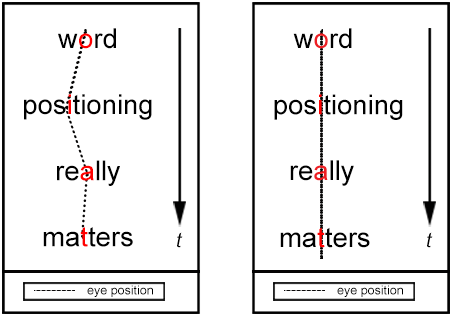
\includegraphics[width=0.4\textwidth]{Pics/opr_spritz}
\caption{Spritz utilizes the optimal recognition position to align words \protect\cite{spritz}.}
\label{fig:spritz_orp}
\end{figure}
\section{Discussion and Conclusion}
When comparing the different reading processes to RSVP, an assumption can be made that RSVP does not allow all reading processes to be used. Skimming and scanning can potentially be used by RSVP, as they only require the ability to recognize single words and transposed words. Rauding requires that the thought of a sentence can be understood, which requires that the reader has time to process the sentence before moving on. If the text is read at rate around the rauding rate - 300 WPM, it should be possible to do with RSVP.   Idea remembering and fact rehearsal, however, cannot be accomplished with RSVP, since they require regression. The possibility of using schema is also excluded, since readers do not have possibility of just reading titles or viewing pictures.

Since RSVP seems to incorporate three different reading processes, process flexibility may be a possibility. According to \cite{spritz}, their RSVP algorithm takes into account the processing time for each word, indicating further that it uses process flexibility. Whether or not the reading efficiency with this RSVP algorithm is the same as when using process flexibility without RSVP remains to be examined.

\citeA{spritz} also claims to increase reading speeds since they are removing the need to saccade, since processing of visual inputs are halted. However, since lexical processing runs in parallel 
to saccadic suppression, a reader can still process text during a saccade. Therefore, the benefits of RSVP might not be to the same degree as previously claimed.

It seems that the idea of RSVP is less well-suited for more complex texts. Sub-vocalization is an integral part of increasing the reading comprehension. Since sub-vocalization follows the speed of how fast the reader is able to speak (about 150 words), it becomes difficult to sub-vocalize when being presented words at a rate of 500 or even 1000 words per minute. 

Spritz and similar speed-reading apps might prove useful for less-complex material, but as stated by \citeA{time_spritz}, if a deeper understanding of a given text is needed, \emph{"reading with an app like Spritz allows us only to read simply, foolishly fast."}



%%%% ---------- How to make headlines and sections ---------- %%%
\section{This is a section} \label{sec:thisSection}
\subsection{This is a subsection}
Let us refer to section \ref{sec:thisSection}.

%%% How to write bold, italics %%%
This text is \textbf{bold}.
This text is \textit{italics}.

%%% ---------- Insert page break ---------- %%%
%%\newpage
%%Here is some text on the next page

%%% ---------- This is how you refer to a figure in the text ---------- %%%
Here is something that I illustrate in figure \ref{fig:wavelength}.

%%% ---------- This is how you insert a single picture ---------- %%%
\begin{figure}[htbp]
\centering
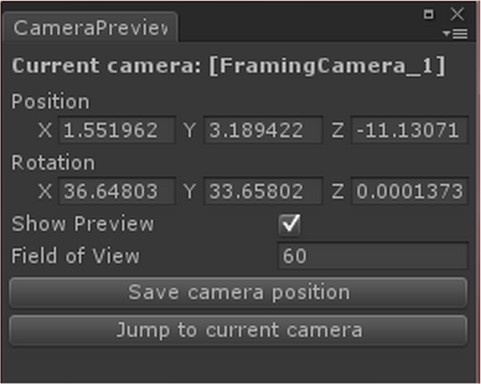
\includegraphics[width=0.50\textwidth]{Pics/Dummy}
\caption{Image caption text goes here bla bla bla bla}
\label{fig:wavelength}
\end{figure}

%%% ---------- This is how you insert multiple pictures ---------- %%%
\begin{figure}[htbp] \centering
\begin{minipage}[b]{0.45\textwidth} \centering
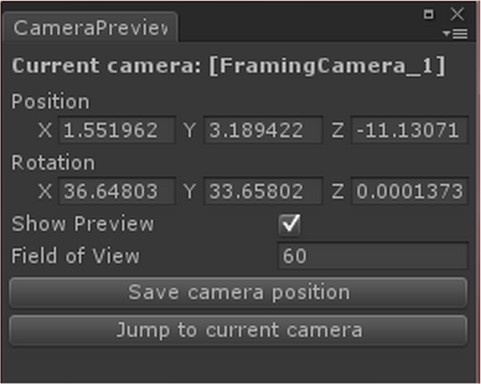
\includegraphics[width=0.60\textwidth]{Pics/Dummy} % Venstre billede
\end{minipage} \hfill
\begin{minipage}[b]{0.45\textwidth} \centering
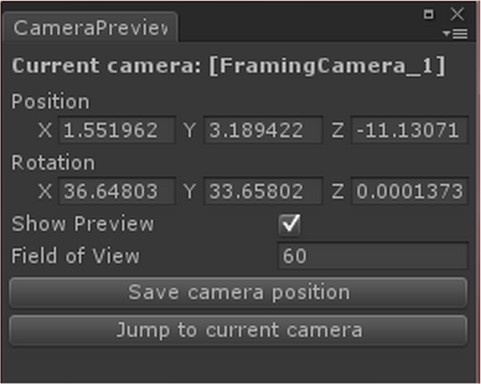
\includegraphics[width=0.60\textwidth]{Pics/Dummy} % Højre billede
\end{minipage} \\ % Captions og labels
\begin{minipage}[t]{0.45\textwidth}
\caption{Caption text for left picture.} % Venstre caption og label
\label{fig:cap1}
\end{minipage} \hfill
\begin{minipage}[t]{0.45\textwidth}
\caption{Caption text for right picture} % Højre caption og label
\label{fig:cap2}
\end{minipage}
\end{figure}

%%% ---------- This is how to make a source reference ---------- %%%
According to bla bla \cite{haigh-hutchinson_real-time_2009} %% passive source
at cite flere: \cite{haigh-hutchinson_real-time_2009, haigh-hutchinson_real-time_2009, haigh-hutchinson_real-time_2009}


%%% ---------- This is how to make bullet points ---------- %%%
\begin{itemize}
\item \textbf{Wavelenght} - Measured in meters from wave top to wave top and denoted as $\lambda$.
\item \textbf{Frequency} - Measured in oscillations per second, Hz, denoted $f$.
\item \textbf{Energy} - Measured in electronvolts, eV, denoted $E$.
\end{itemize}

%%% ---------- This is how to do math stuff ---------- %%%
To derive the wavelength or the frequency, formula \ref{eq:wavelenght} is applied:
\begin{align}
\centering 
\lambda = \frac{C}{f}
\label{eq:wavelenght} 
\end{align}
where {$C$} is the speed of light.



%%% This is how to make footnotes %%%
Hello, I need a footnote \footnote[0]{You can read me, no?}.

%%% This is how to insert a table %%%
\begin{table}[htbp]
\centering
\begin{tabular}{|l|c|c|}
\hline
& Personer
& Totalpris \\\hline
Lasagne
& 4
& 160
\\\hline
Flødekartofler
& 6
& 210
\\\hline
\end{tabular}
\caption{Valg af mad.}
\label{tab:mums}
\end{table} %% GUSTAV'S GUIDE: look at this for how to insert figures, quotes, etc.
\bibliography{references}
%\bibliography{sample}
\end{document}
